% !TEX root=talk.tex
\section[Introduction]{What are \TeX, \LaTeX\ and Friends?}

%--------------------------------------------------------------------
%--- The FYP
%--------------------------------------------------------------------

\begin{frame}[fragile]
\setlength{\fboxsep}{0.333em}
\frametitle{The Final Year Project}
Is $50$--$70$ pages long and contains
\pause

\begin{itemize}
\item Mathematical equations\hspace{1em}\framebox{$\displaystyle\int_{-\infty}^\infty e^{-x^2} \,\mathrm{d}x = \sqrt{\pi}$}
\pause

\item Graphs
\hspace{18em}\raisebox{0pt}[0pt][0pt]{\framebox{
\begin{tikzpicture}[scale=0.5, baseline=1.25]
  \draw[->,>={Stealth[length={4pt}]}] (-2,0) -- (2,0);
  \draw[->,>={Stealth[length={4pt}]}] (0,-.5) -- (0,2);

  \clip (-2,-.5) rectangle (2,2);

  \draw plot[parametric, domain=-2:2, samples=100] function {t, t**3-t+0.5};
\end{tikzpicture}
}}
\pause

\item Tables
\hspace{1em}\raisebox{0em}[2em][2em]{
\framebox{
\begin{tabular}{lccc}
$x$ & 0 & 1 & 2 \\ \midrule
$y$ & 0.5 & 0.5 & 7.5
\end{tabular}}}
\pause

\item Source code
\hspace{0.5em}\begin{minipage}{8em}
\begin{lstlisting}[frame=single,language=matlab,lineskip=-2pt,
basicstyle=\ttfamily,
commentstyle=\upshape\sffamily\small\color{SeaGreen4},keepspaces=true,
keywordstyle=\bfseries\color{Maroon},stringstyle=\rmfamily\color{Sienna2}]
if x > 0
    y = sqrt(x);
end
\end{lstlisting}
\end{minipage}
\pause

\item References and a bibliography
\hspace{2em}\raisebox{1em}[0em][2em]{\framebox{
\begin{minipage}{13em}
\textsmaller{\rmfamily\noindent
See [1, Theorem~1.2.6] for a proof.
\smallskip

[1] S.~Abbott. \emph{Understanding Analysis}. \\
Undergraduate Texts in Mathematics. Springer, New York, 2015.}
\end{minipage}}}
\end{itemize}
\end{frame}

% %--------------------------------------------------------------------
% %--- Ever Worried about These?
% %--------------------------------------------------------------------

% \begin{frame}
% \frametitle{Ever Worried about These?}
% \begin{itemize}
% \item<2-12,13> Is my introduction good enough?
% \item<3-12,14|alert@14|trans:alert@1|handout:alert@1> My math equations don't display correctly.
% \item<4-12,13> Should this discussion go into this section or that one?
% \item<5-12,14|alert@14|trans:alert@1|handout:alert@1> What formatting did I use for my subsection headings again?
% \item<6-12,14|alert@14|trans:alert@1|handout:alert@1> My section/figure/page numbering has gone all wrong!
% \item<7-12,13> Should I split this section into two?
% \item<8-12,14|alert@14|trans:alert@1|handout:alert@1> My citation formatting got inconsistent.
% \item<9-12,14|alert@14|trans:alert@1|handout:alert@1> My citations and bibliography aren't synchronised!
% \item<10-12,13> What results should I put in this table?
% \item<11-12,14|alert@14|trans:alert@1|handout:alert@1> Oops, I forgot to update the table of contents.
% \item<12,14|alert@14|trans:alert@1|handout:alert@1> Should I think some more about the conclusions section?
% \end{itemize}
% \end{frame}

%--------------------------------------------------------------------
%--- Tex, LaTeX, and Friends
%--------------------------------------------------------------------

\begin{frame}<1>[label=texNfriends]
\frametitle{What are \TeX\ and \LaTeX,\ and Friends?}

\begin{description}
\item<1>[\TeX] 
\begin{itemize}
\item From Greek $\uptau\upepsilon\upchi$. \\
Abbreviation of $\uptau\upepsilon\upchi\upnu\upeta$, meaning \emph{art} or \emph{craft}.
\item \textsmaller{ASCII} \texttt{TeX}, \textsmaller{\textipa{/tEx/}, \textipa{/tEk/}}.
\item A \structure{computer typesetting system} created by Donald Knuth
for `the creation of beautiful books'. First release 1978. (39 years ago!)
\end{itemize}


\item<2>[\LaTeX]
\begin{itemize}
\item A shortening of `Lamport-\TeX'.
\item \textsmaller{ASCII} \texttt{LaTeX}, \textsmaller{\textipa{/"leItEx/}, \textipa{/"leItEk/}, \textipa{/"lA:tEx/}, \textipa{/"lA:tEk/}}.
\item A \structure{document preparation system} by Leslie Lamport. First release 1985.
	\end{itemize}

\item <3>[Friends]
\begin{itemize}
\item \structure{Bib\TeX}, \structure{Biber}, \structure{MakeIndex}, \ldots
\item \url{http://www.ctan.org/what_is_tex.html}
\end{itemize}
\end{description}
\end{frame}

%--------------------------------------------------------------------
%--- Knuth and Lamport
%--------------------------------------------------------------------

{\setbeamertemplate{background canvas}{\hskip-2em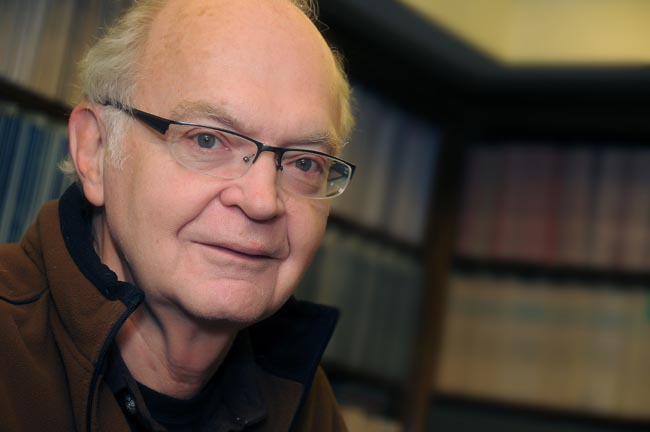
\includegraphics[height=\paperheight]{images/d_knuth_noticia}}
\setbeamercolor{itemize item}{fg=structure.fg!45}
\begin{frame}[plain,t]
\vfill
\hfill
\begin{minipage}{.42\textwidth}
\usebeamercolor[bg]{normal text}
\hspace{1em}\textbf{\large Donald Knuth (1938--)}
\begin{itemize}
\usebeamercolor[bg]{normal text}
\item American computer scientist, mathematician, and professor emeritus at Stanford University
\item Author of the multi-volume work \emph{The Art of Computer Programming}
\item ``Father of the analysis of algorithms''
\end{itemize}
\end{minipage}

\bigskip

\begin{quote}
\usebeamercolor[bg]{normal text}
``Science is what we understand well enough to explain to a computer. Art is everything else we do.''

\medskip

``If you optimize everything, you will always be unhappy.''
\end{quote}
\vspace*{-4\baselineskip}\null
\end{frame}}

\mode<beamer>{
  \againframe<2>{texNfriends}
}

{\setbeamertemplate{background canvas}{%
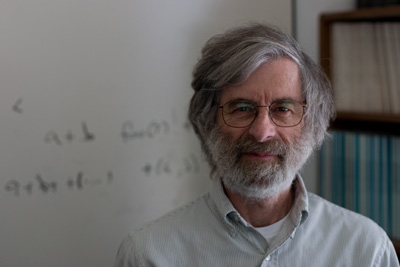
\includegraphics[height=\paperheight]{images/lamport}}
\setbeamercolor{itemize item}{fg=structure.fg!45}
\begin{frame}[plain,t]
\vfill
\begin{minipage}{.45\textwidth}
\usebeamercolor[bg]{normal text}
\hspace{1em}\textbf{\large Leslie Lamport (1941--)}
\begin{itemize}
\usebeamercolor[bg]{normal text}
\item American computer scientist
\item Laid the foundations of the theory of distributed systems
\end{itemize}

\bigskip

\emph{
\usebeamercolor[bg]{normal text}
``A distributed system is one in which the failure of a computer you didn't even know existed can render your own computer unusable.''}
\end{minipage}
\end{frame}
}

\mode<beamer>{
  \againframe<3->{texNfriends}
}

%--------------------------------------------------------------------
%--- Typesetting and Word Processing
%--------------------------------------------------------------------

\begin{frame}
\frametitle{Typesetting and Word Processing}
\framesubtitle{Apples and Oranges}

\begin{columns}[T]
\begin{column}{.5\textwidth}
\textlarger{\structure{Word Processors}} \\
\textsmaller{Word, Google Docs, LibreOffice}
\begin{itemize}
\item What you see is what you get.
\item Content and layout are generated at the same time.
\item Local style adjustments are easier to make.
\end{itemize}
\end{column}

\onslide<3>
\begin{column}{.5\textwidth}
\textlarger{\structure{Typesetting Software}} \\
\textsmaller{\LaTeX, InDesign, Scribus}
\begin{itemize}
\item Separation of content and presentation.
\item Layout can be globally optimised.
\item Uniform style easier to realise.
\end{itemize}
\end{column}
\end{columns}

\onslide<2->
\begin{cvarblock}[0.82\textwidth]{}
\textbf{typesetting} \emph{n}. The activity of arranging printed text and images on the page when preparing a book, newspaper, etc. for printing.
\hfill\textsmaller{(Cambridge English Dictionary)}
\end{cvarblock}

\end{frame}

%--------------------------------------------------------------------
%--- Scalability
%--------------------------------------------------------------------

\begin{frame}
\frametitle{Scalability}
\bigskip

\centering
\begin{tikzpicture}
  %\draw[help lines,gray!20] (0,0) grid (6,4);
  %\draw[semithick] (0,0) rectangle (6,4);
  \draw[semithick,->,>=latex'] (-.5, 0) -- (6.5, 0);
  \draw[semithick,->,>=latex'] (0, -.5) -- (0,5);
  \draw[dashed,structure.fg!50!black,semithick] 
    (0, 0.2) parabola (3.5,4)
      node[above, font=\footnotesize, text=black]{Impossible to do} (3.5, 4);
  \node[left] at (3,3) {MS Word};
  \draw[structure.fg!50!black,semithick] (0, 1) parabola (6,3); 
  \node at (5.2,2) {\LaTeX};
  \node[below,font=\footnotesize] at (3,0) {Document complexity and size};
  \node[xshift=-8pt, yshift=4pt, font=\footnotesize, transform shape, rotate=90] 
    at (0,2.2) {Effort and time consumption};
\end{tikzpicture}

\begin{center}
Scalability of \LaTeX\ and Microsoft Word as a function of \\
document size and complexity.
\end{center}

\btVFill

\hfill
\textsmaller{
Redrawn from Marko Pinteric's original \structure{\href{http://www.pinteric.com/miktex.html}{(link)}}.}
\medskip

\end{frame}

%--------------------------------------------------------------------
%--- Example .tex File
%--------------------------------------------------------------------

% TODO: Add creation of first-en.pdf file & cropping automatic
% TODO: See original file for swapping languages example

\begin{frame}[fragile]
\frametitle{Example \texttt{.tex} File}
\setlength{\fboxsep}{.5em}

\begin{columns}[T]
\begin{column}{.48\textwidth}
\begin{beamerboxesrounded}[width=\linewidth]{}
\vspace{-1em}
\begin{lstlisting}[moretexcs={maketitle,tableofcontents,subsection},
emph={document,abstract,babel},
basicstyle={\ttfamily\footnotesize\lsstyle},lineskip=-2pt]
\documentclass[a4paper,11pt]{article}
\author{Martins Bruveris}
\title{An Introductory Paper}
\date{\today}
\usepackage[english]{babel}

\begin{document}
\maketitle
\tableofcontents

\begin{abstract}
This paper introduces\ldots
\end{abstract}

\section{Introduction}
We consider\ldots

\section{State of the Art}
We look at\ldots

\subsection{Document Formats}
There are many\ldots
\end{document}
\end{lstlisting}
\vspace{-1em}
\end{beamerboxesrounded}
\end{column}

\begin{column}{.48\textwidth}
\uncover<3>{%
\hfill\fcolorbox{black}{white}{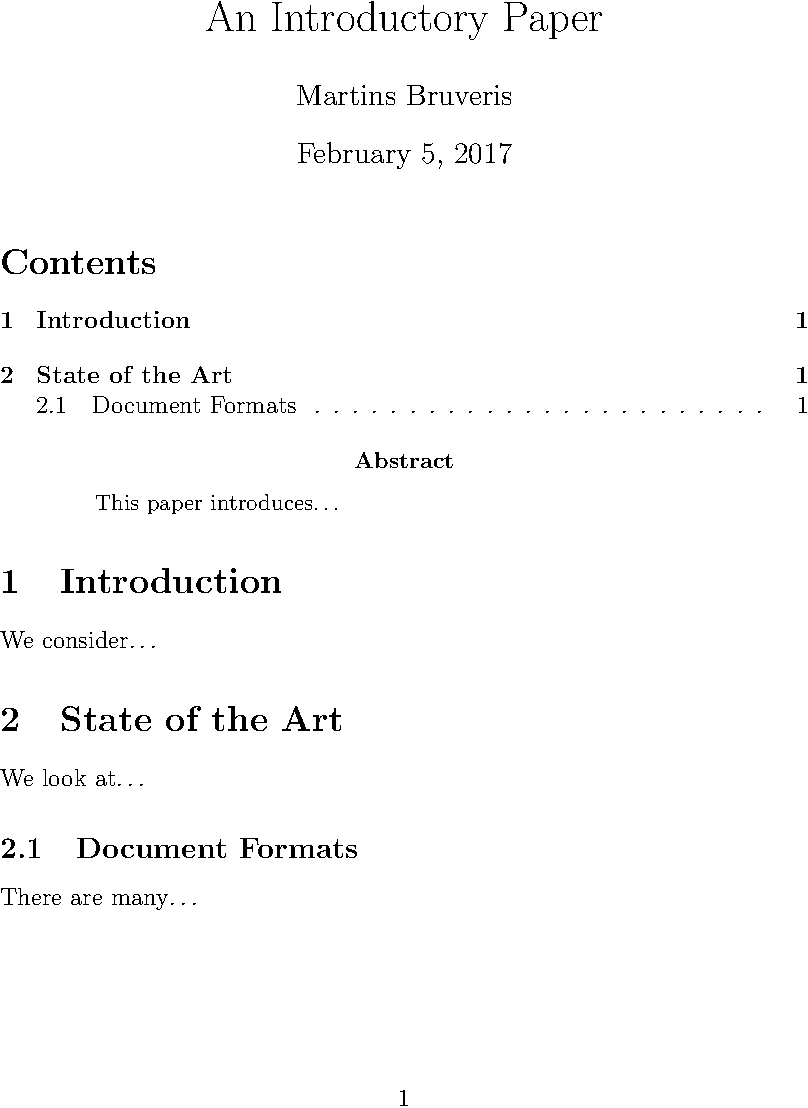
\includegraphics[width=0.94\linewidth]{examples/first-en}}
}
\end{column}
\end{columns}

\uncover<2->{%
\begin{tikzpicture}[remember picture,overlay]
\node[single arrow,fill=DarkSeaGreen,font=\ttfamily\bfseries,xshift=-1em] at (current page.center) {pdflatex};
\end{tikzpicture}
}

\end{frame}

%--------------------------------------------------------------------
%--- Module structure
%--------------------------------------------------------------------

\begin{frame}
\frametitle{Module Structure}

\begin{description}
\setlength\labelwidth{8.5em}
\setlength\itemindent{3em}
\item[Lecture]
Introduction to \LaTeX\ (happening right now)
\pause\medskip

\item[Labs]
Three computer labs for each group (W21--23) \\
\hspace{\itemindent}Mon, Tue or Thu 17--19 in HALB 213
\pause\medskip

\item[Assignment]
Preparing a document, about two pages long \\
\hspace{\itemindent} Thematically connected to MA2895 assignment \\
\hspace{\itemindent} Due 3 April 2017 (TBC)
\pause\medskip

\item[Assessment]
Contributes 20\% towards MA2812

\end{description}

\end{frame}

%--------------------------------------------------------------------
%--- Where Do I Get It?
%--------------------------------------------------------------------

\begin{frame}
\frametitle{Where Do I Get It?}
\begin{description}
\setlength\labelwidth{8.5em}
\setlength\itemindent{3em}
\item[Online]
ShareLaTeX (\url{www.sharelatex.com}) \\ 
\hspace{\itemindent}Overleaf (\url{www.overleaf.com})
\pause
\medskip
\item[Windows] Mik\TeX, \TeX Live
\item[Linux] \TeX Live
\item[Mac OS X] Mac\TeX\ (based on \TeX Live)
\pause
\medskip
\item[Editors]
TeXmaker, TeXworks, TeXstudio, emacs \\
\hspace{\itemindent}(Mac OS X) TeXShop
\pause
\medskip
\item[\hologo{LaTeX} Packages] Use Mik\TeX\ or \TeX Live's package manager
\pause
\medskip
\item[Documentation] 
(Online) \url{http://texdoc.net/pkg/<package name>}\\
\hspace{\itemindent}(\TeX Live) \texttt{\$ texdoc <package name>}\\
\hspace{\itemindent}(Mik\TeX) \texttt{\$ mthelp <package name>}
\end{description}
\end{frame}

%--------------------------------------------------------------------
%--- Where Can I Find Help?
%--------------------------------------------------------------------

\begin{frame}
\frametitle{Where Can I Find Help?}

\begin{description}
\setlength\labelwidth{7em}
\setlength\itemindent{1em}
\item[Online]
Search the internet \\
\hspace{\itemindent}%
\textsmaller{E.g. use `latex add table of contents' in your favorite search engine.} \\
\hspace{\itemindent}\TeX\ Stack Exchange 
\textsmaller{(\url{http://tex.stackexchange.com})} \\
\hspace{\itemindent}The \LaTeX\ Wikibook 
\textsmaller{ (\url{http://en.wikibooks.org/wiki/latex})}
\medskip
\pause

\item[Books]
George Graetzer, \emph{Practical \LaTeX}. Springer, 2014. \\
\hspace{\itemindent}\textsmaller{Electronic version available through the library.
\href{http://lib.myilibrary.com/Open.aspx?id=644795&src=0}{%
{\usebeamercolor[fg]{description item} (Link)}}} \\
\hspace{\itemindent}%
Helmut Kopka, Patric W.~Daley, \emph{Guide to \LaTeX}. \\
\hspace{\itemindent}Fourth Edition. Addison-Wesley, 2004. \\
\hspace{\itemindent}\textsmaller{Electronic version available through the library.
\href{http://lib.myilibrary.com/Open.aspx?id=243269&src=0}{%
{\usebeamercolor[fg]{description item} (Link)}}} \\
\medskip
\pause

\item[Other]
\LaTeX\ Cheat Sheet 
\href{https://wch.github.io/latexsheet/}{%
{\usebeamercolor[fg]{description item} \textsmaller{(Link)}}} \\
\hspace{\itemindent}The Not So Short Introduction to \LaTeXe
\href{http://tug.ctan.org/info/lshort/english/lshort.pdf}{%
{\usebeamercolor[fg]{description item} \textsmaller{(Link)}}} \\
\hspace{\itemindent}The ShareLaTeX Documentation
\href{https://www.sharelatex.com/learn}{%
{\usebeamercolor[fg]{description item} \textsmaller{(Link)}}} \\
\hspace{\itemindent}Overleaf \LaTeX Tutorial
\href{https://www.overleaf.com/latex/learn/free-online-introduction-to-latex-part-1}{%
{\usebeamercolor[fg]{description item} \textsmaller{(Link)}}}
\end{description}
\end{frame}

%--------------------------------------------------------------------
%--- Why use LaTeX
%--------------------------------------------------------------------

\begin{frame}
\frametitle{Why?}
\framesubtitle{From \url{http://www.ctan.org/what_is_tex.html}}
\begin{columns}[T]
\begin{column}{.48\textwidth}
\begin{varblock}<1->{Output Quality}
\begin{itemize}
\item Professional quality output.
\item It knows typesetting.
\end{itemize}
\end{varblock}

\begin{varblock}<2->{Superior Engineering}
\begin{itemize}
\item It's fast.
\item It's stable.
\item It's extensible.
\item Plain text input.
\item Many output types.
\end{itemize}
\end{varblock}
\end{column}

\begin{column}{.48\textwidth}
\begin{varblock}<3->{Freedom}
\begin{itemize}
\item It's free.
\item It runs anywhere.
\end{itemize}
\end{varblock}

\begin{varblock}<4->{Popularity}
\begin{itemize}
\item It's standard in academia and science.
\end{itemize}
\end{varblock}
\end{column}
\end{columns}
\end{frame}

%%% Local Variables:
%%% TeX-master: "talk"
%%% End:
